\section{General background}
\label{sec:background}

\subsection{Potential fields due to 3D sources}
\label{sec:potential_fields_3D_sources}

Consider a topocentric Cartesian coordinate system with axes 
$x$, $y$, and $z$ pointing to north, east and down, respectively.
In this system, let a set of 3D gravity or magnetic sources be defined over a closed region 
$\overline{\mathcal{V}'}$ located in the subsurface, with top limited by a vertical 
coordinate $z^{t}_{0}$.
The closed region $\overline{\mathcal{V}'}$ is defined as the union of a finite collection of $N_{\nu}$ 
disjoint regular regions $\mathcal{V}'_{\nu}$ and their respective boundaries $\partial\mathcal{V}'_{\nu}$, that is, 
$\overline{\mathcal{V}'} = \bigcup_{\nu = 1}^{N_{\nu}} \overline{\mathcal{V}'_{\nu}}$, where
$\overline{\mathcal{V}'_{\nu}} = \mathcal{V}'_{\nu} \cup \partial\mathcal{V}'_{\nu}$.
Each regular region $\mathcal{V}'_{\nu}$ is an open, connected subset of $\mathbb{R}^{3}$, with boundary 
defined by a closed and compact surface $\partial \mathcal{V}'_{\nu}$ free of double points 
\citep[][p. 22]{freeden_gerhards2012}.

The potential field produced by the 3D sources at observation points 
$\mathbf{r} = (x, y, z)^{\top}$ (Fig. \ref{fig:Figure1}) is represented by:
\begin{equation}
	d^{o}(\mathbf{r}) = D_{d} \, U(\mathbf{r}) \: , 
	\quad \mathbf{r} \notin \overline{\mathcal{V}'} \: ,
	\label{eq:observed-data-space}
\end{equation}
where $D_{d}$ is a space-domain differential operator acting on the Newtonian potential
\begin{equation}
	U(\mathbf{r}) = \kappa \iiint\limits_{\overline{\mathcal{V}'}}
	\sigma(\mathbf{r}') \: \frac{1}{\| \mathbf{r} - \mathbf{r}'\|}
	\: d\mathcal{V}' \: , 
	\quad \mathbf{r} \notin \overline{\mathcal{V}'} \: ,
	\label{eq:potential-U-space}
\end{equation}
$\kappa$ is a proportionality constant,
$\tfrac{1}{\| \mathbf{r} - \mathbf{r}' \|}$ is the inverse distance function
between the observation point $\mathbf{r}$ and a point 
$\mathbf{r}' = (x', y', z')^{\top} \in \overline{\mathcal{V}'}$
and $\sigma$ is the scalar function representing 
the density (contrast) or total-magnetization intensity within the sources.
We consider that $\sigma$ is 
(i) $\gamma$-Hölder continuous with exponent $\gamma \in (0, 1]$ 
\citep[][p. 14]{freeden_gerhards2012} within each regular region $\mathcal{V}'_{\nu}$ up to its corresponding boundary 
$\partial\mathcal{V}'_{\nu}$ and (ii) admits bounded step discontinuities across the boundaries $\partial\mathcal{V}'_{\nu}$ 
so that it is zero at all points $\mathbf{r} \notin \overline{\mathcal{V}'}$.
These conditions on $\sigma$ guarantee that the second partial derivatives of the Newtonian potential $U$ exist and 
are continuous inside each regular region $\mathcal{V}'_{\nu}$ forming $\overline{\mathcal{V}'}$.

Throughout the text, we use the notation $\mathcal{F} [ \cdot ]$ to define a 
two-dimensional Fourier transform of a generic scalar function computed on a horizontal plane, with respect to
the spatial coordinates $x$ and $y$. To simplify the notation, we conveniently omit its dependence 
on the wavenumbers $k_{x}$ and $k_{y}$.
By using this notation, we define the Fourier transform of the potential field 
$d^{o}$ (Eq. \ref{eq:observed-data-space}) at points 
$\mathbf{r}^{\dagger} = (x^{\dagger}, y^{\dagger}, z^{\dagger}_{0})^{\top}$ 
on a horizontal surface $\mathcal{S}^{\dagger}$ with constant vertical coordinate $z^{\dagger}_{0}$ above the 
sources (Fig. \ref{fig:Figure1}) by \citep[e.g.,][]{bhattacharyya1967,gunn1975}:
\begin{equation}
	\mathcal{F} [ d^{o}(\mathbf{r}^{\dagger}) ] =
	\alpha_{d} \, \mathcal{F} [ U(\mathbf{r}^{\dagger}) ] \: ,
	\quad \mathbf{r}^{\dagger} \in \mathcal{S}^{\dagger} \: ,
	\label{eq:observed-data-Fourier}
\end{equation}
where 
\begin{equation}
	\mathcal{F} [ U(\mathbf{r}^{\dagger}) ] = 2 \pi \kappa 
	\int\limits_{z^{t}_{0}}^{\infty}
	\mathcal{F} [ \sigma(\mathbf{r}') ] \:
	\frac{e^{- k \, (z' - z^{\dagger}_{0})}}{k}
	\: dz' \: , 
	\quad \mathbf{r}^{\dagger} \in \mathcal{S}^{\dagger} \: ,
	\label{eq:potential-U-Fourier}
\end{equation}
is the Fourier transform of the Newtonian potential 
$U$ (Eq. \ref{eq:potential-U-space}) on $\mathcal{S}^{\dagger}$, 
$k = \sqrt{k_{x}^{2} + k_{y}^{2}}$, and
\begin{equation}
	\mathcal{F} [ \sigma(\mathbf{r}') ] = 
	\int\limits_{-\infty}^{\infty}\int\limits_{-\infty}^{\infty}
	\sigma(\mathbf{r}') \: e^{-\mathtt{i} \, (k_{x} \, x' + k_{y} \, y')}
	\: dx'dy'
	\label{eq:sigma-Fourier}
\end{equation}
is the Fourier transform of $\sigma$ on the horizontal plane at the vertical
coordinate $z'$ and $\mathtt{i}$ represents the imaginary unit.

In Eq. \ref{eq:observed-data-Fourier}, $\alpha_{d}$ is a function of the 
wavenumbers $k_{x}$ and $k_{y}$ and represents the differential operator 
$D_{d}$ (Eq. \ref{eq:observed-data-space}) in the Fourier domain.
In the subsequent developments, the relationship that enables the derivation of the Fourier-domain 
operator $\alpha_{d}$ from its space-domain counterpart $D_{d}$ and vice-versa is given by
\begin{equation}
	D(\ell, \hat{\mathbf{u}}) = 
	\left( \hat{\mathbf{u}}^{\top} \nabla \right)^{\ell} \Leftrightarrow
	\alpha(\ell, \hat{\mathbf{u}}) = \left( \hat{\mathbf{u}}^{\top} \mathbf{k} \right)^{\ell} \: ,
	\quad \ell \in \{ 0, 1, 2 \} \: ,
	\label{eq:diff-operators-generic}
\end{equation}
where $\hat{\mathbf{u}}$ is a constant unit vector,
$\nabla$ is the vector differential operator nabla and 
$\mathbf{k} = ( \mathtt{i} \, k_{x} \, , \, \mathtt{i} \, k_{y} \, , \, k)^{\top}$
\cite{pedersen1978}.
The differential operator $D$ (Eq. \ref{eq:diff-operators-generic})
has a symbolic form based on that used by \cite[][p. 179]{kaplan2002}.

By combining successive applications of $D$ 
(Eq. \ref{eq:diff-operators-generic}) with properly chosen $\ell$ and $\hat{\mathbf{u}}$, 
we may define differential operators leading to different potential fields commonly used 
in Geophysics (Table \ref{tbl:Table1}).
Using $\ell = 0$ leads to $D(0, \hat{\mathbf{u}}) = \alpha(0, \hat{\mathbf{u}}) = 1$ that produces 
no differentiation.
With $\ell = 1$ and a constant unit vector $\hat{\mathbf{u}}$ we define the following
directional derivative of first order
\begin{equation}
	D(1, \hat{\mathbf{u}}) \, U(\mathbf{r}) = \nabla U(\mathbf{r})^{\top} \hat{\mathbf{u}} \: ,
	\label{eq:potential-U-oblique-1st-deriv-space}
\end{equation}
where
\begin{equation}
	\nabla U(\mathbf{r}) = \left( 
	\tfrac{\partial}{\partial x} U(\mathbf{r}),
	\tfrac{\partial}{\partial y} U(\mathbf{r}),
	\tfrac{\partial}{\partial z} U(\mathbf{r}) \right)^{\top}
	\label{eq:potential-U-grad-space}
\end{equation}
is the gradient of $U$ (Eq. \ref{eq:potential-U-space}), with elements
given by the partial derivatives of first order
\begin{equation}
	\tfrac{\partial}{\partial u} U(\mathbf{r}) = \kappa \iiint\limits_{\overline{\mathcal{V}'}}
	\sigma(\mathbf{r}') \: 
	\tfrac{\partial}{\partial u} \left( \frac{1}{\| \mathbf{r} - \mathbf{r}'\|} \right)
	\: d\mathcal{V}' \: , 
	\quad \mathbf{r} \notin \overline{\mathcal{V}'} \: , \quad u \in \{ x, y, z \} \: .
	\label{eq:potential-U-1st-deriv-space}
\end{equation}
The first-order directional derivative (Eq. \ref{eq:potential-U-oblique-1st-deriv-space})
coincides with the partial derivatives of first order $\tfrac{\partial}{\partial u} U$ (Eq. \ref{eq:potential-U-1st-deriv-space})
for the particular case in which the unit vector $\hat{\mathbf{u}}$ coincides with one of the canonical base vectors
\begin{equation}
	\hat{\mathbf{x}} = (1,0,0)^{\top} , \quad 
	\hat{\mathbf{y}} = (0,1,0)^{\top} , \quad
	\hat{\mathbf{z}} = (0,0,1)^{\top} \: .
	\label{eq:canonical-base-vector}
\end{equation}
For example, $D(1, \hat{\mathbf{z}}) \, U(\mathbf{r}) = \tfrac{\partial}{\partial z} U(\mathbf{r})$.

It can also be verified from Eq. \ref{eq:diff-operators-generic} that 
\begin{equation}
	D(1, \hat{\mathbf{u}}) \, D(1, \hat{\mathbf{v}}) \, U(\mathbf{r}) = 
	\hat{\mathbf{u}}^{\top} \mathbf{H}_{U}(\mathbf{r}) \, \hat{\mathbf{v}} \: ,
	\label{eq:potential-U-oblique-2nd-deriv-space}
\end{equation}
represents a second-order directional derivative along constant unit vectors $\hat{\mathbf{u}}$ and
$\hat{\mathbf{v}}$, where 
\begin{equation}
	\mathbf{H}_{U}(\mathbf{r}) = 
	\begin{bmatrix}
		\tfrac{\partial^{2}}{\partial x^{2}} U(\mathbf{r}) & 
		\tfrac{\partial^{2}}{\partial x \, \partial y} U(\mathbf{r}) & 
		\tfrac{\partial^{2}}{\partial x \, \partial z} U(\mathbf{r}) \\
		\tfrac{\partial^{2}}{\partial x \, \partial y} U(\mathbf{r}) & 
		\tfrac{\partial^{2}}{\partial y^{2}} U(\mathbf{r}) & 
		\tfrac{\partial^{2}}{\partial y \, \partial z} U(\mathbf{r}) \\
		\tfrac{\partial^{2}}{\partial x \, \partial z} U(\mathbf{r}) & 
		\tfrac{\partial^{2}}{\partial y \, \partial z} U(\mathbf{r}) & 
		\tfrac{\partial^{2}}{\partial z^{2}} U(\mathbf{r})
	\end{bmatrix}
	\label{eq:potential-U-Hessian}
\end{equation}
is the Hessian matrix \citep[e.g.,][p. 158]{kaplan2002} of $U$ (Eq. \ref{eq:potential-U-space}),
with elements given by the partial derivatives of second order
\begin{equation}
	\tfrac{\partial^{2}}{\partial u \, \partial v} U(\mathbf{r}) = \kappa \iiint\limits_{\overline{\mathcal{V}'}}
	\sigma(\mathbf{r}') \: 
	\tfrac{\partial^{2}}{\partial u \, \partial v} \left( \frac{1}{\| \mathbf{r} - \mathbf{r}'\|} \right)
	\: d\mathcal{V}' \: , \quad \mathbf{r} \notin \overline{\mathcal{V}'} \: , \quad u, v \in \{ x, y, z \} \: .
	\label{eq:potential-U-2nd-deriv-space}
\end{equation} 
Finally, it can also be verified that the second-order directional derivative given by Eq. 
\ref{eq:potential-U-oblique-2nd-deriv-space} coincides with the partial derivatives of second order 
$\tfrac{\partial^{2}}{\partial u \, \partial v} U$ (Eq. \ref{eq:potential-U-2nd-deriv-space}) for the particular 
cases in which the unit vectors $\hat{\mathbf{u}}$ and $\hat{\mathbf{v}}$ are given by the canonical base vectors 
(Eq. \ref{eq:canonical-base-vector}). For example,
$D(1, \hat{\mathbf{x}}) \, D(1, \hat{\mathbf{y}}) \, U(\mathbf{r}) = \tfrac{\partial^{2}}{\partial x \, \partial y} U(\mathbf{r})$.


\subsection{Classical Dirichlet's and Neumann's problems on a plane}
\label{subsec:dirichlet_neumann}

Due to the properties imposed on $\sigma$ (Eq. \ref{eq:potential-U-space}), the potential 
$U$ has continuous partial derivatives of all orders, 
satisfies the Laplace's equation at all points $\mathbf{r} \notin \overline{\mathcal{V}'}$ 
located outside the sources, as well as is regular at infinity \citep[][p. 122--124, 217]{kellogg1967}.
Because of these properties, we have that
\begin{equation}
	U(\mathbf{r}) = 
	\int\limits_{-\infty}^{\infty} \int\limits_{-\infty}^{\infty}
	D(\ell, \hat{\mathbf{z}}) U(\mathbf{r}'') \:\: 
	D(1 - \ell, \hat{\mathbf{z}}) \Psi(\mathbf{r}, \mathbf{r}'')
	\: d\mathcal{S}'' \: , \quad  z < z''_{0} < z^{t}_{0} \: ,
	\quad \ell \in \{0, 1\} \: ,
	\label{eq:U-Dirichlet-Neumann}
\end{equation}
where $\mathbf{r} = (x, y, z)^{\top} \notin \overline{\mathcal{V}'}$; 
$\mathbf{r}'' = (x'', y'', z''_{0})^{\top} \in \mathcal{S}''$ (Fig. \ref{fig:Figure1}); 
$D(\ell, \hat{\mathbf{z}})$ is the space-domain differential operator 
defined by Eq. \ref{eq:diff-operators-generic} in terms of the canonical base vector 
$\hat{\mathbf{z}}$ (Eq. \ref{eq:canonical-base-vector}) and 
\begin{equation}
	\Psi(\mathbf{r}, \mathbf{r}'') = 
	\frac{1}{2\pi} \: 
	\frac{1}{\| \mathbf{r} - \mathbf{r}'' \|} \: , 
	\quad \mathbf{r} \ne \mathbf{r}'' \: ,
	\label{eq:Psi}
\end{equation}
represents the scaled inverse distance function between $\mathbf{r}$ and $\mathbf{r}''$. 
Equation \ref{eq:U-Dirichlet-Neumann} is commonly deduced from 
the ``Green's third identity'' \citep[][p. 219]{kellogg1967}, according to
the general outline presented by \cite{roy1962}, for example.

For $\ell = 0$, Eq. \ref{eq:U-Dirichlet-Neumann} states that $U$ can be defined
in terms of its values $D(0, \hat{\mathbf{z}}) U(\mathbf{r}'') = U(\mathbf{r}'')$ on a horizontal surface $\mathcal{S}''$ 
above the sources and represents the solution of the classical ``Dirichlet’s problem'' or the 
``first boundary value problem of potential theory'' \citep[][p. 236]{kellogg1967} on a plane, where 
$D(1, \hat{\mathbf{z}}) \Psi(\mathbf{r}, \mathbf{r}'') = \tfrac{\partial}{\partial z} \Psi(\mathbf{r}, \mathbf{r}'')$ 
represents the Green's function.
From the physical point of view, Eq. \ref{eq:U-Dirichlet-Neumann} with $\ell = 0$ defines a continuous 
layer of monopoles (or vertically-magnetized dipoles) that is located on $\mathcal{S}''$, has 
physical-property distribution $U(\mathbf{r}'')$ and exactly reproduces the 
potential field $U$ at any point $\mathbf{r}$ above $\mathcal{S}''$.

On the other hand, Eq. \ref{eq:U-Dirichlet-Neumann} for $\ell = 1$ shows that $U$ can also
be defined in terms of its vertical derivative 
$D(1, \hat{\mathbf{z}}) U(\mathbf{r}'') = \tfrac{\partial}{\partial z} U(\mathbf{r}'')$ 
on a horizontal surface $\mathcal{S}''$ above the sources and represents the solution of the classical ``Neumann’s problem'' or the 
``second boundary value problem of potential theory'' \citep[][p. 246]{kellogg1967} on a plane, 
with the Green's function given by $D(0, \hat{\mathbf{u}}) \Psi(\mathbf{r}, \mathbf{r}'') = \Psi(\mathbf{r}, \mathbf{r}'')$.
Equation \ref{eq:U-Dirichlet-Neumann} with $\ell = 1$ can be alternatively interpreted as a planar layer of
vertically-magnetized dipoles (or monopoles) that is located on $\mathcal{S}''$, has 
physical-property distribution $\tfrac{\partial}{\partial z} U(\mathbf{r}'')$ and exactly reproduces 
$U$ at any point $\mathbf{r}$ above $\mathcal{S}''$.

By applying the Fourier-convolution theorem \citep[][p. 268]{blakely1996} to Eq. \ref{eq:U-Dirichlet-Neumann} 
on a horizontal surface $\mathcal{S}^{\dagger}$ above the sources, we find that
\begin{equation}
	\mathcal{F} [ U(\mathbf{r}^{\dagger}) ] = 
	k \: \mathcal{F} [ U(\mathbf{r}'') ] \:
	\mathcal{F} [ \Psi(\mathbf{r}^{\dagger}, \mathbf{r}'') ] \: ,
	\quad z^{\dagger}_{0} < z''_{0} < z^{t}_{0} \: , \quad k \ne 0 \: ,
	\label{eq:U-Dirichlet-Neumann-Fourier}
\end{equation}
where $\mathbf{r}^{\dagger} = (x^{\dagger}, y^{\dagger}, z^{\dagger}_{0})^{\top} \in \mathcal{S}^{\dagger}$; 
$\mathbf{r}'' = (x'', y'', z''_{0})^{\top} \in \mathcal{S}''$ (Fig. \ref{fig:Figure1}) and
\begin{equation}
	\mathcal{F} [ \Psi(\mathbf{r}^{\dagger}, \mathbf{r}'') ] 
	= \frac{e^{- k \, (z''_{0} - z^{\dagger}_{0})}}{k}
	\: , \quad z^{\dagger}_{0} < z''_{0} \: , \quad k \ne 0 \: ,
	\label{eq:Psi-Fourier}
\end{equation}
is defined according to \citep[][p. 275]{blakely1996}.

\subsection{Potential-field transformations}
\label{subsec:potential_field_transformations}

Several geophysical applications use the observed potential field 
$d^{o}$ (Eq. \ref{eq:observed-data-space}) to estimate another potential field 
defined in the space domain by
\begin{equation}
	f(\mathbf{r}) = D_{f} \, U(\mathbf{r}) \: , 
	\quad \mathbf{r} \notin \overline{\mathcal{V}'} \: ,
	\label{eq:transformed-field-space}
\end{equation}
or, in the Fourier domain, 
\begin{equation}
	\mathcal{F} [ f(\mathbf{r}^{\dagger}) ] =
	\alpha_{f} \, \mathcal{F} [ U(\mathbf{r}^{\dagger}) ] \: ,
	\quad \mathbf{r}^{\dagger} \in \mathcal{S}^{\dagger} \: ,
	\label{eq:transformed-field-Fourier}
\end{equation}
where $\mathcal{S}^{\dagger}$ is a horizontal surface defined above the sources (Fig. \ref{fig:Figure1});
$D_{f}$ is a space-domain differential operator acting on $U$ (Eq. \ref{eq:potential-U-space}) and
$\alpha_{f}$ its corresponding representation in the Fourier domain.
The differential operators $D_{f}$ and $\alpha_{f}$ associated with the potential field 
$f$ (Eq(s). \ref{eq:transformed-field-space} and \ref{eq:transformed-field-Fourier}) are commonly
defined in terms of $D$ and $\alpha$ (Eq. \ref{eq:diff-operators-generic}). 
Estimating $f$ (Eq(s). \ref{eq:transformed-field-space} and \ref{eq:transformed-field-Fourier}) from 
the observed potential field $d^{o}$ (Eq. \ref{eq:observed-data-space}) is an operation 
commonly known in geophysics as ``potential-field transformation''.

A common approach to compute potential-field transformations \citep[e.g.,][]{gunn1975} 
consists in using the definition of observed data in the Fourier domain (Eq. \ref{eq:observed-data-Fourier}) 
and manipulating the Fourier domain solution of the Dirichlet's and Neumann's problems 
(Eq. \ref{eq:U-Dirichlet-Neumann-Fourier}) to obtain
\begin{equation}
	\mathcal{F} [ f(\mathbf{r}^{\dagger}) ] =
	\left( \tfrac{\alpha_{f}}{\alpha_{d}} \right) \, \mathcal{F} \left[ d^{o}(\mathbf{r}^{\dagger}) \right] \: , 
	\quad \mathbf{r}^{\dagger} \in \mathcal{S}^{\dagger} \: .
	\label{eq:field-transformation-Fourier}
\end{equation}
Equation \ref{eq:field-transformation-Fourier} defines a single-step potential-field transformation 
in terms of the observed potential field $d^{o}$ on a planar surface $\mathcal{S}^{\dagger}$ 
located above the sources, at $z^{\dagger}_{0}$ (Fig. \ref{fig:Figure1}). 
The potential field $f$ in the space domain is obtained by simply computing the inverse Fourier 
transform of \ref{eq:field-transformation-Fourier}.
For simplicity, both fields $d^o$ and $f$ are defined at the same points in Eq. \ref{eq:field-transformation-Fourier}, 
although it's worth noting that, in certain geophysical contexts, $f$ may be estimated at different locations from 
where potential-field data were measured.

The ``equivalent-layer technique'' offers an alternative approach that is generally defined in the 
space domain to compute potential-field transformations. What follows aims at discussing the well-established 
empirical approaches used in the equivalent-layer technique, as well as discussing the theoretical background 
supporting them.

\begin{table}[h]
	\caption{Relevant potential fields for geophysical applications.}
		\renewcommand{\arraystretch}{0.8}
		\begin{tabular}{%
			>{\small\centering}m{0.15\textwidth}
			>{\footnotesize\setlength{\baselineskip}{0.5\baselineskip}\centering}m{0.25\textwidth}
			>{\tiny\setlength{\baselineskip}{0.5\baselineskip}\raggedright\arraybackslash}m{0.60\textwidth}
		}
		\toprule%
		{\small \textbf{Symbol}} & 
		{\small \textbf{Potential field}} & 
		{\small \textbf{Brief description}} \\
		\midrule%
		$U$ & 
		Newtonian potential &
		In gravity applications, $U$ (Eq. \ref{eq:potential-U-space}) represents the gravitational potential. 
		In magnetic applications, it represents an auxiliary potential whose first directional derivative along the 
		constant magnetization direction of the sources gives the magnetic scalar potential. \\
		$\tfrac{\partial}{\partial u} U$ &
		Gravitational attraction component or pseudogravity anomaly &
		First derivative of $U$ along the Cartesian directions $u \in \{ x, y, z \}$ (Eq. \ref{eq:potential-U-1st-deriv-space}). 
		In gravity applications, the vertical component $\tfrac{\partial}{\partial z} U$ 
		is called ``gravity disturbance'' \citep[e.g.,][p. 93]{hofmann-wellenhof-moritz2005}. 
		The debate around the differences between gravity anomaly and gravity disturbance is beyond the scope of the 
		present work and has been carried about from a more geodetic than a geophysical point of view 
		\citep[e.g.,][]{li2001, fairhead2003, hackney-featherstone2003, hinze2005, vajda-etal2006, vajda-etal2007, vajda-etal2008}. 
		In magnetic applications, the vertical 
		component represents the ``pseudogravity anomaly'' 
		\citep[][p. 345]{blakely1996}. \\
		$\tfrac{\partial^{2}}{\partial u \, \partial v} U$ &
		Gravitational tensor component or RTP anomaly &
		Second derivative of $U$ along the Cartesian directions $u, v \in \{ x, y, z \}$ 
		(Eq. \ref{eq:potential-U-2nd-deriv-space}). 
		In gravity applications, the second derivative represents a component of the 
		``gravitational tensor'' \citep[e.g.,][]{pedersen_rasmussen1990}.
		In magnetic applications, the particular second derivative 
		$\tfrac{\partial^{2}}{\partial z^{2}} U$ along the vertical 
		direction represents the ``RTP anomaly''. 
		Differently from generic total-field anomalies 
		\citep[e.g.,][p. 178]{blakely1996}, which have a ``skewed'' pattern 
		oscillating from negative to positive values and do not have their maxima placed 
		right above the magnetic sources, the RTP anomaly is easier to interpret 
		because it is predominantly positive right above the sources and
		decays to zero towards their boundaries. \cite{baranov1957} was the first
		to propose a method, called ``reduction to the pole'' (RTP), to transform 
		generic total-field anomalies into this special anomaly. \\
		$-\nabla U^{\top} \hat{\mathbf{v}}$ &
		Magnetic scalar potential &
		Directional derivative of $U$ along the constant magnetization direction $\hat{\mathbf{v}}$ of the sources 
		(Eq. \ref{eq:potential-U-oblique-1st-deriv-space}), where $\nabla U$ is the gradient of 
		$U$ (Eq. \ref{eq:potential-U-grad-space}). \\
		$\hat{\mathbf{u}}^{\top} \mathbf{H}_{U} \, \hat{\mathbf{v}}$ &
		Magnetic induction field component &
		Directional derivative of $U$ along $\hat{\mathbf{v}}$, the constant magnetization direction of the sources, 
		and $\hat{\mathbf{u}}$ (Eq. \ref{eq:potential-U-oblique-2nd-deriv-space}), where $\mathbf{H}_{U}$ is the 
		Hessian of $U$ (Eq. \ref{eq:potential-U-Hessian}). For the case in which 
		$\hat{\mathbf{u}}$ is $\hat{\mathbf{x}}$, $\hat{\mathbf{y}}$ or $\hat{\mathbf{z}}$ (Eq. \ref{eq:canonical-base-vector}),
		the directional derivative represents a Cartesian component of the magnetic induction field. 
		For the case in which $\hat{\mathbf{u}}$ is the constant direction of the main field, the directional derivative 
		represents the ``approximated total-field anomaly'' \citep[e.g.,][p. 179]{blakely1996}. \\
		$\| \nabla \left[\nabla U^{\top} \hat{\mathbf{v}}\right] \|_{2}$ &
		Amplitude of the magnetic induction field &
		Square root of the sum of the squares of the Cartesian magnetic induction field components. This field, also known as 
		``amplitude of the anomalous magnetic field'' \citep{li_etal2010} or 
		``amplitude of the magnetic anomaly vector'' \citep{hidalgo_gato_etal2021, melo_etal2021}, has a weak dependence on 
		the total-magnetization direction of the
		true sources. \\
		\botrule%
	\end{tabular}
	\label{tbl:Table1}
\end{table}

\begin{figure}[h]
	\centering
	\noindent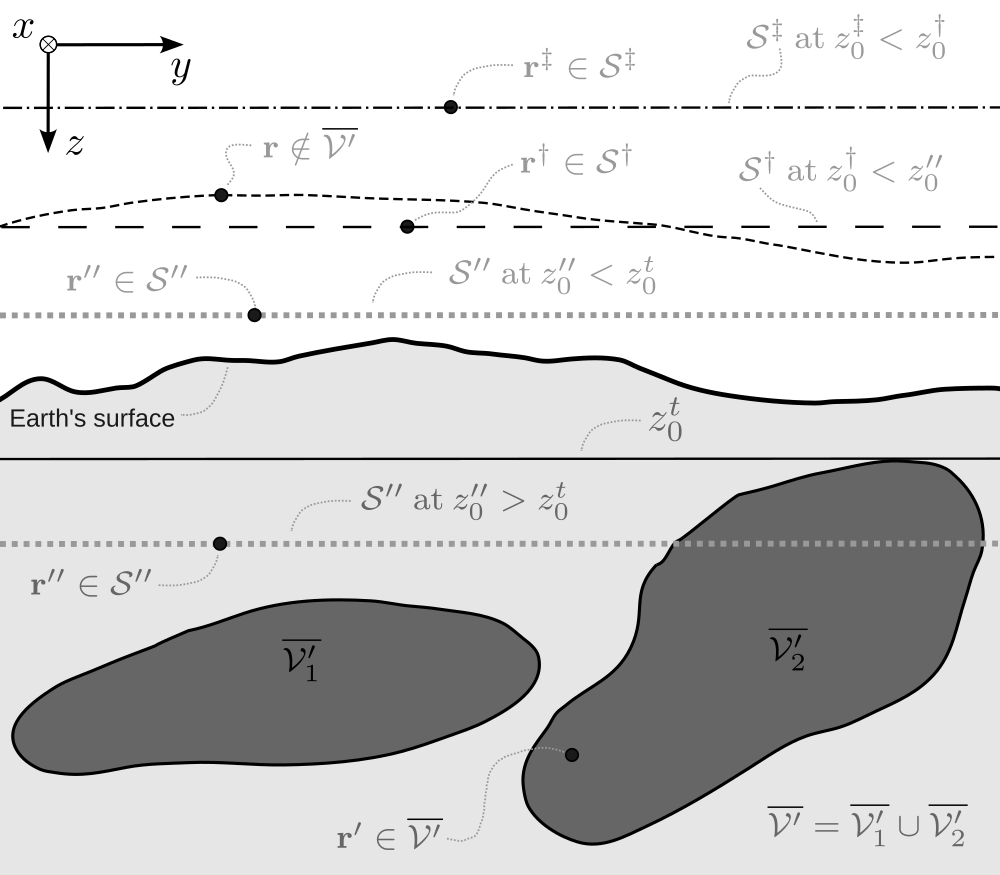
\includegraphics[width=0.8\textwidth]{Figure1_1.png}
	\caption{%
		2D schematic representation of a vertical $yz$ plane crossing the sources (represented in dark gray),
		with $x$ axis pointing inward the page (represented by the ``$\otimes$" symbol).
		The sources are located in the subsurface (represented in light gray), over a 
		closed region $\overline{\mathcal{V}'}$ formed by $N_{\nu} = 2$ disjoint closed regions 
		$\overline{\mathcal{V}'_{\nu}}$, $\nu \in \{1, 2\}$, with top limited by the plane $z^{t}_{0}$. 
		The fine dashed lines represent two possible horizontal surfaces $\mathcal{S}''$, one located 
		at $z''_{0} < z^{t}_{0}$, above the sources, and another at $z''_{0} > z^{t}_{0}$, crossing the sources.
		The medium dashed line represents the surface containing the observation points 
		$\mathbf{r}$, all above $\mathcal{S}''$.
		The long dashed line represents a planar surface $\mathcal{S}^{\dagger}$ located 
		at $z^{\dagger}_{0} < z''_{0}$.
		Finally, the dashed-dot line represents a planar surface $\mathcal{S}^{\ddagger}$ located 
		at $z^{\ddagger}_{0} < z^{\dagger}_{0}$.
	}
	\label{fig:Figure1}
\end{figure}